%\section{Systemmodelle}
\newpage
\subsection{Anwendungsfalldiagramm}
Das System ist in die Benutzer*gruppe Benutzer*, Betreuer* und Admin* unterteilt. Folgendes Use-Case-Diagramm beschreibt die Interaktionsmöglichkeiten der einzelnen Benutzer*gruppe mit dem Server:
\begin{itemize}
	\item Mit dem Accounts Verwalten kann der Admin* neuen Benutzer* anlegen, Account abändern, Rechte vergeben oder löschen.
	\item Mit Komponente Login können Benutzer* sich anmelden bzw. abmelden.
	\item Eine Benutzer* kann neue Zeiterfassung starten. Nachträgliche Erfassung, Bearbeitung oder Korrektur ist möglich. Er darf seine eigene erfasste Zeiten und Stundenzettel ansehen. Er kann Warnungen und Erinnerungen lesen. Er druckt sein Stundenzettel aus, unterschreibt und gibt es bei seinem Betreuer* ab.
	\item Ein Betreuer* darf die Erfasste Zeiten, Stundenzettel, und Nachrichten von allen seinen zugewiesenen Benutzern* ansehen. Er kontrolliert Stundenzettel von seinen Benutzern* und gibt die Status weiter an den Admin*.
	\item Der Admin* darf alles ansehen. Außderdem sammelt er noch alle Stundenzettel ein.
\end{itemize}


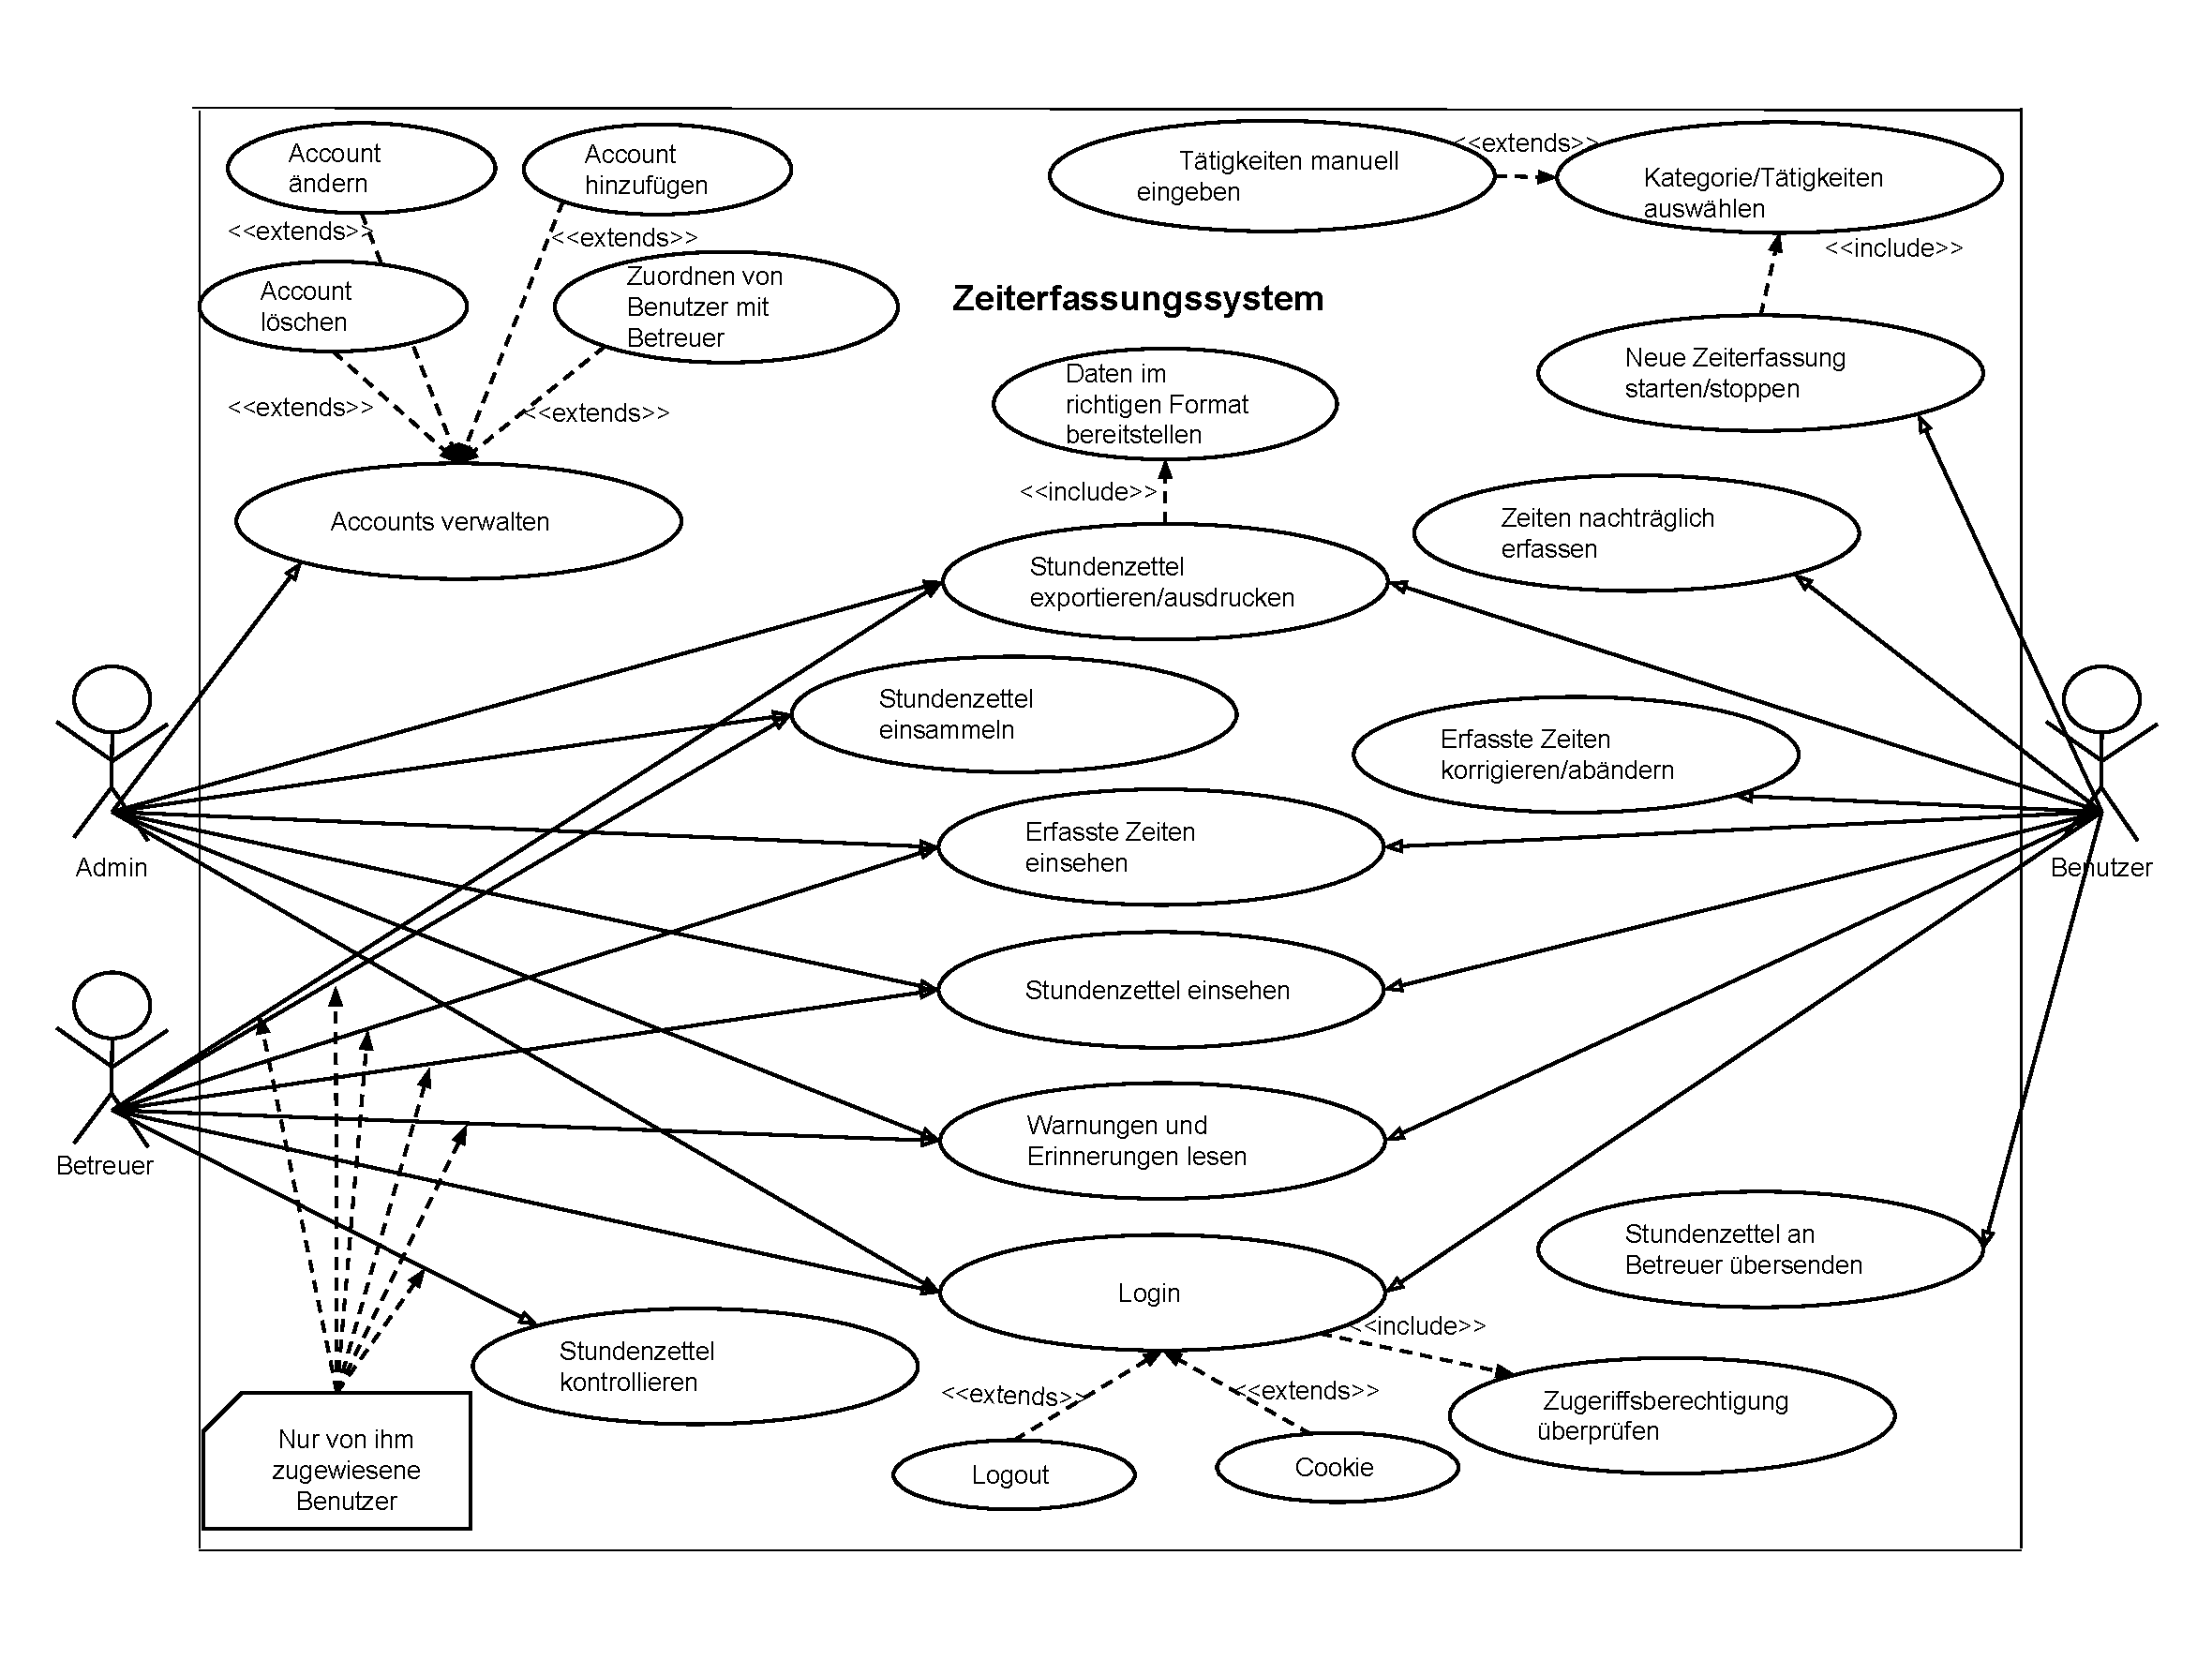
\includegraphics[width=\linewidth]{Anwendungsfalldiagramm.pdf}\\
